\section{Appendix}

\begin{figure}[h!tb] 
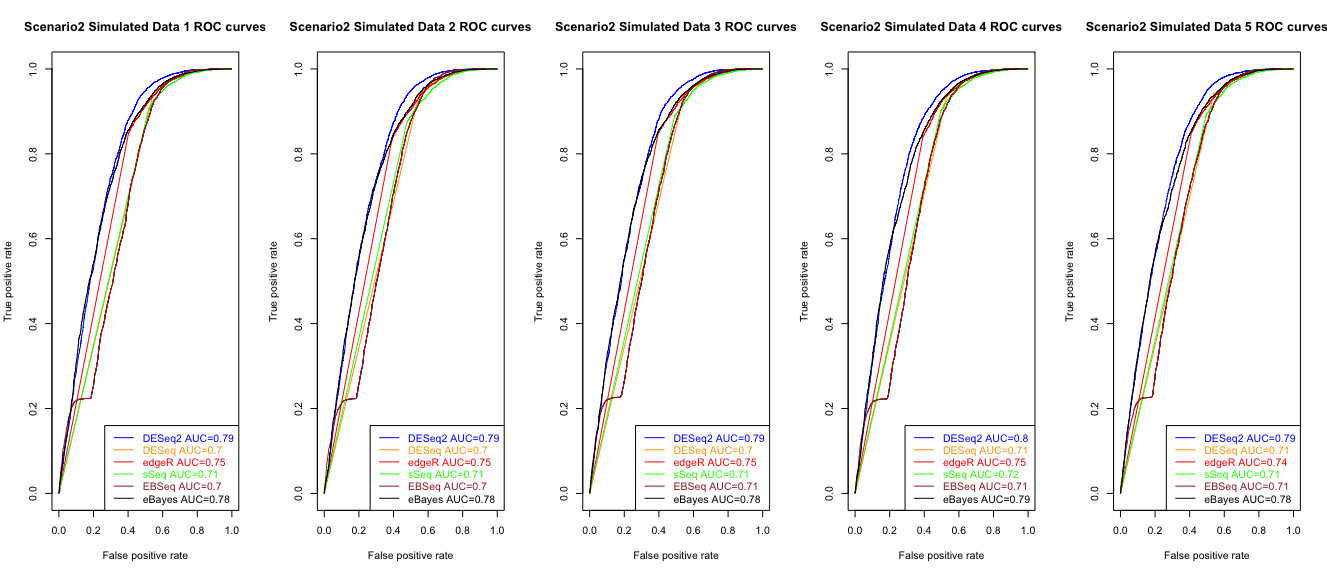
\includegraphics[height=6cm,width=15cm]{sc2_roc}
\caption{ROC curves of Simulated Datasets with $nGenes=10000, nSamples=8, pDiff=30\%$}
\label{sc2_roc}
\end{figure}

\begin{figure}[h!tb] 
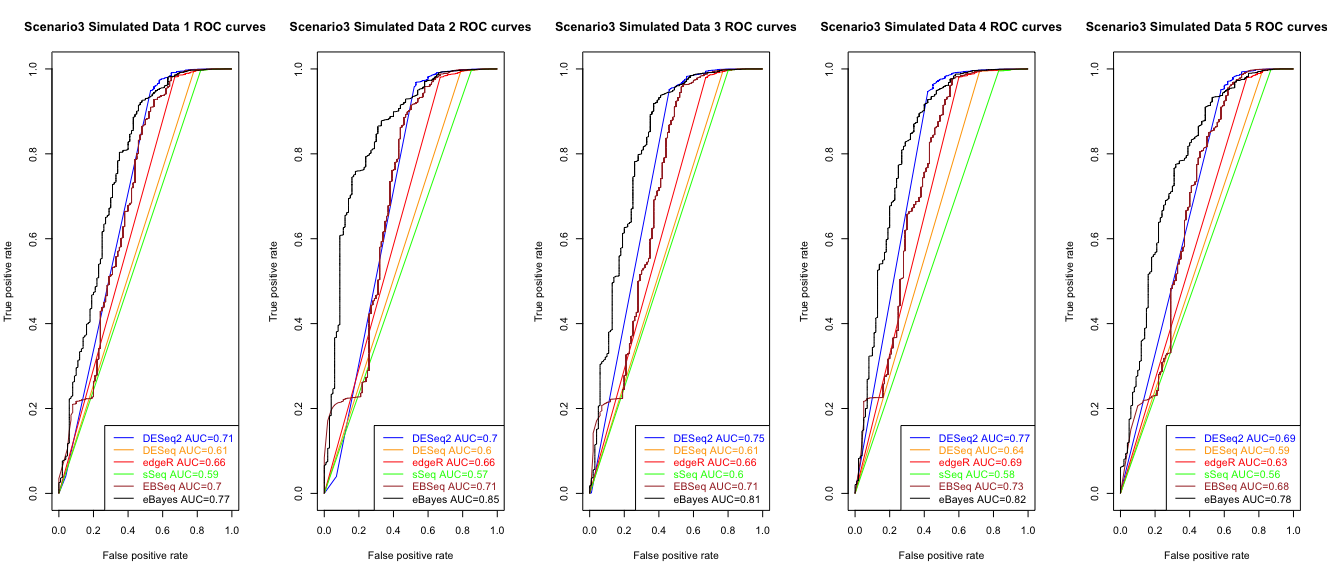
\includegraphics[height=6cm,width=15cm]{sc3_roc}
\caption{ROC curves of Simulated Datasets with $nGenes=10000, nSamples=8, pDiff=1\%$}
\label{sc3_roc}
\end{figure}


\begin{figure}[h!tb] 
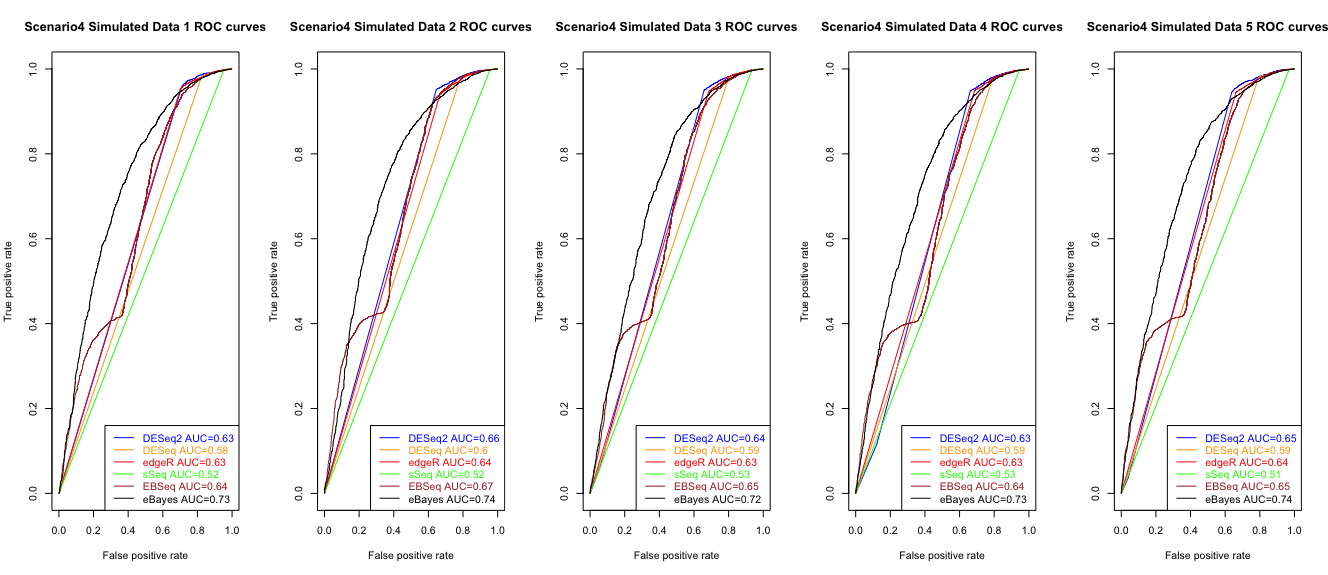
\includegraphics[height=6cm,width=15cm]{sc4_roc}
\caption{ROC curves of Simulated Datasets with $nGenes=10000, nSamples=4, pDiff=10\%$}
\label{sc4_roc}
\end{figure}


\begin{figure}[h!tb] 
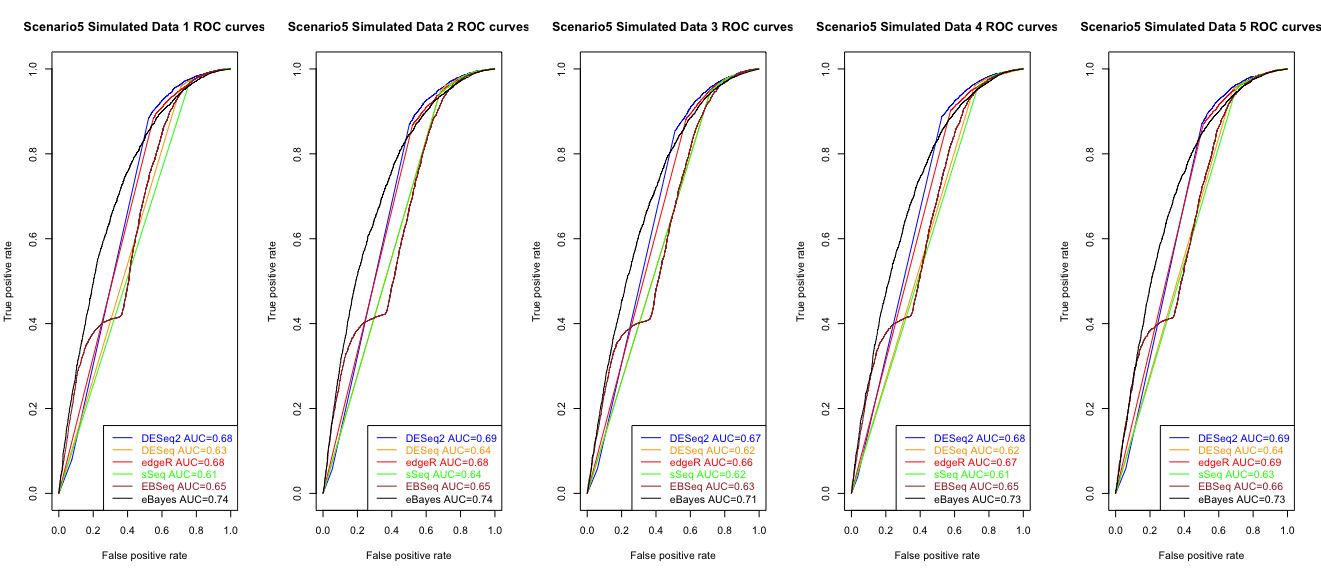
\includegraphics[height=6cm,width=15cm]{sc5_roc}
\caption{ROC curves of Simulated Datasets with $nGenes=10000, nSamples=4, pDiff=30\%$}
\label{sc5_roc}
\end{figure}


\begin{figure}[h!tb] 
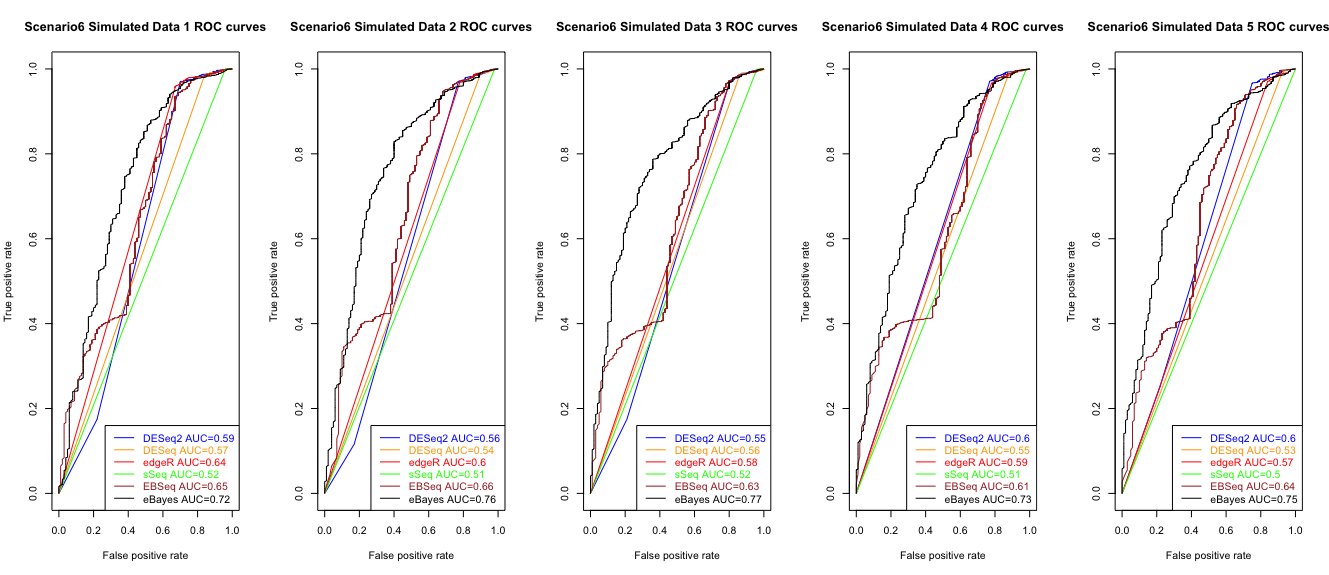
\includegraphics[height=6cm,width=15cm]{sc6_roc}
\caption{ROC curves of Simulated Datasets with $nGenes=10000, nSamples=4, pDiff=1\%$}
\label{sc6_roc}
\end{figure}

\begin{figure}[h!tb] 
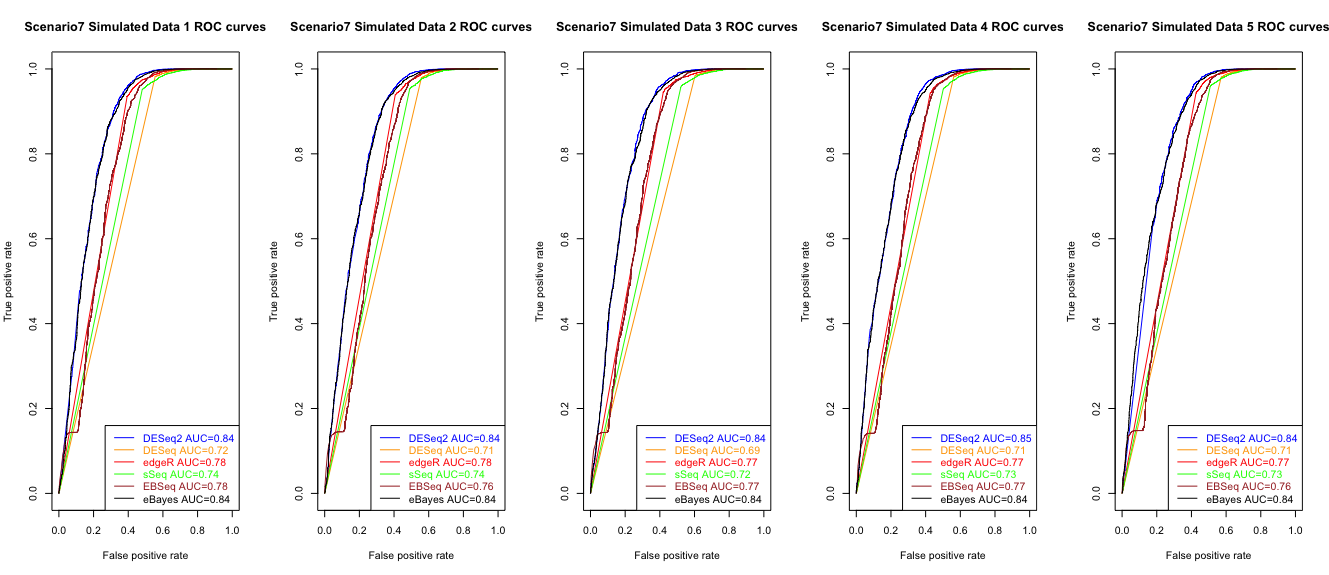
\includegraphics[height=6cm,width=15cm]{sc7_roc}
\caption{ROC curves of Simulated Datasets with $nGenes=10000, nSamples=16, pDiff=10\%$}
\label{sc7_roc}
\end{figure}

\begin{figure}[h!tb] 
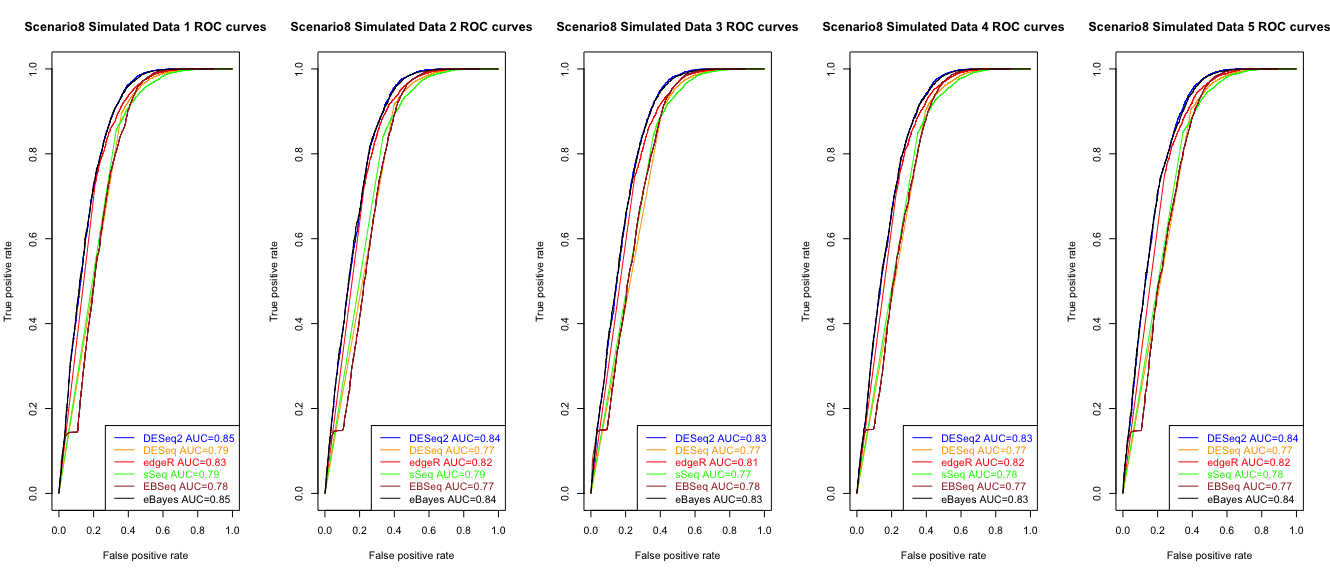
\includegraphics[height=6cm,width=15cm]{sc8_roc}
\caption{ROC curves of Simulated Datasets with $nGenes=10000, nSamples=16, pDiff=30\%$}
\label{sc8_roc}
\end{figure}

\begin{figure}[h!tb] 
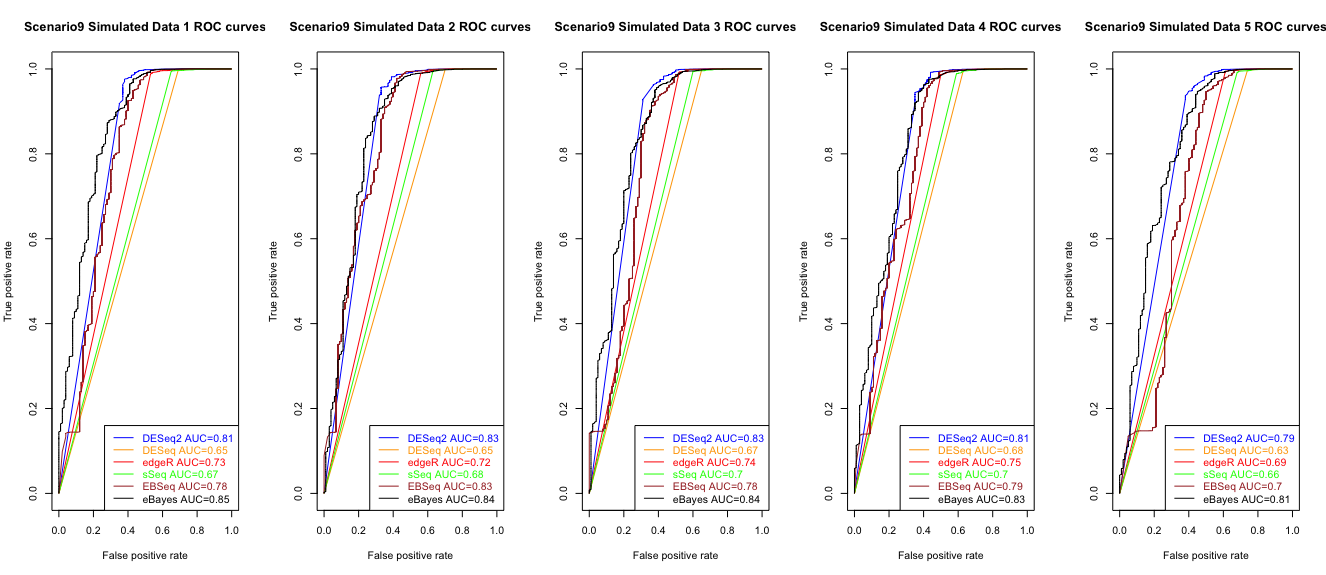
\includegraphics[height=6cm,width=15cm]{sc9_roc}
\caption{ROC curves of Simulated Datasets with $nGenes=10000, nSamples=16, pDiff=1\%$}
\label{sc9_roc}
\end{figure}


\begin{figure}[h!tb] 
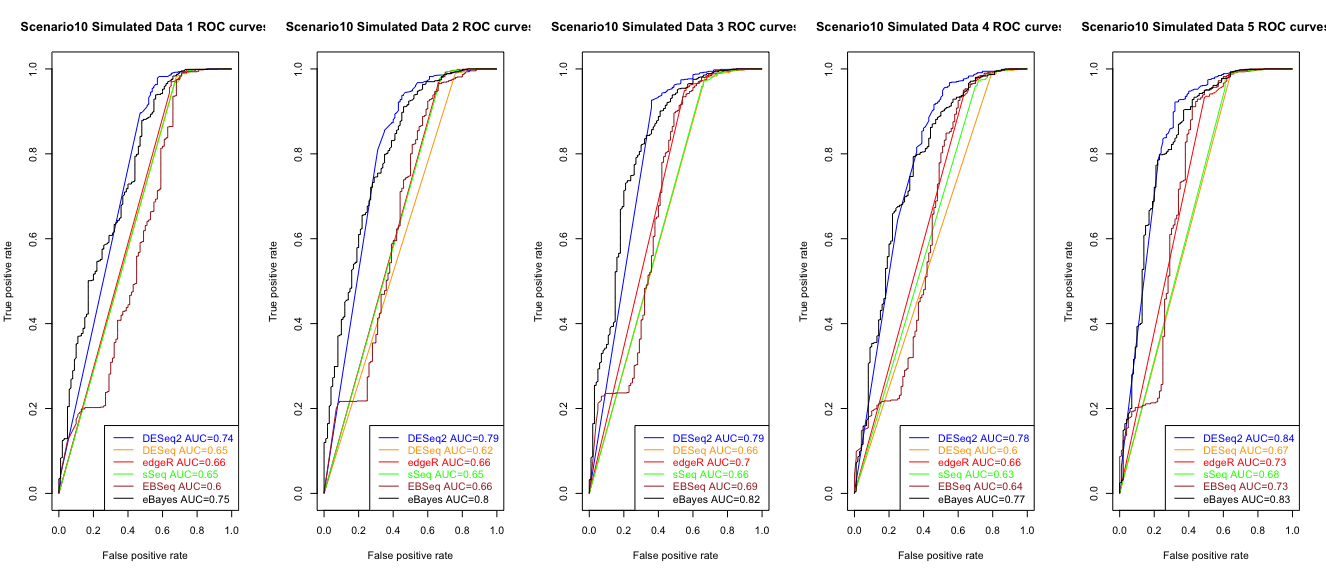
\includegraphics[height=6cm,width=15cm]{sc10_roc}
\caption{ROC curves of Simulated Datasets with $nGenes=1000, nSamples=8, pDiff=10\%$}
\label{sc10_roc}
\end{figure}




\begin{figure}[h!tb] 
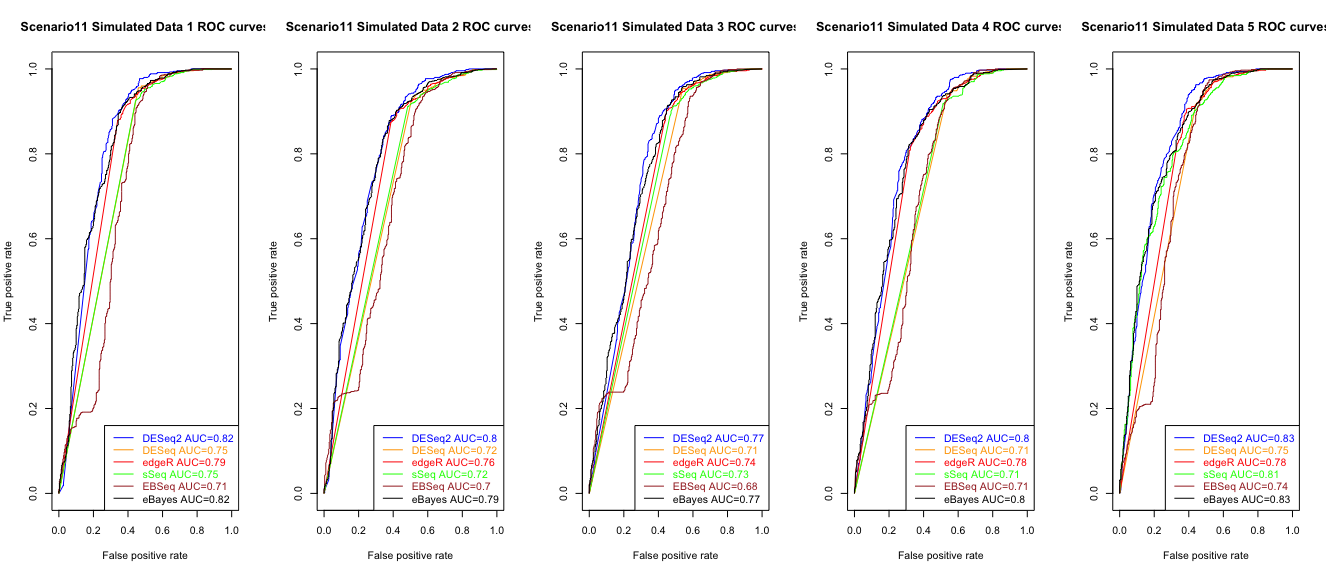
\includegraphics[height=6cm,width=15cm]{sc11_roc}
\caption{ROC curves of Simulated Datasets with $nGenes=1000, nSamples=8, pDiff=30\%$}
\label{sc11_roc}
\end{figure}

\begin{figure}[h!tb] 
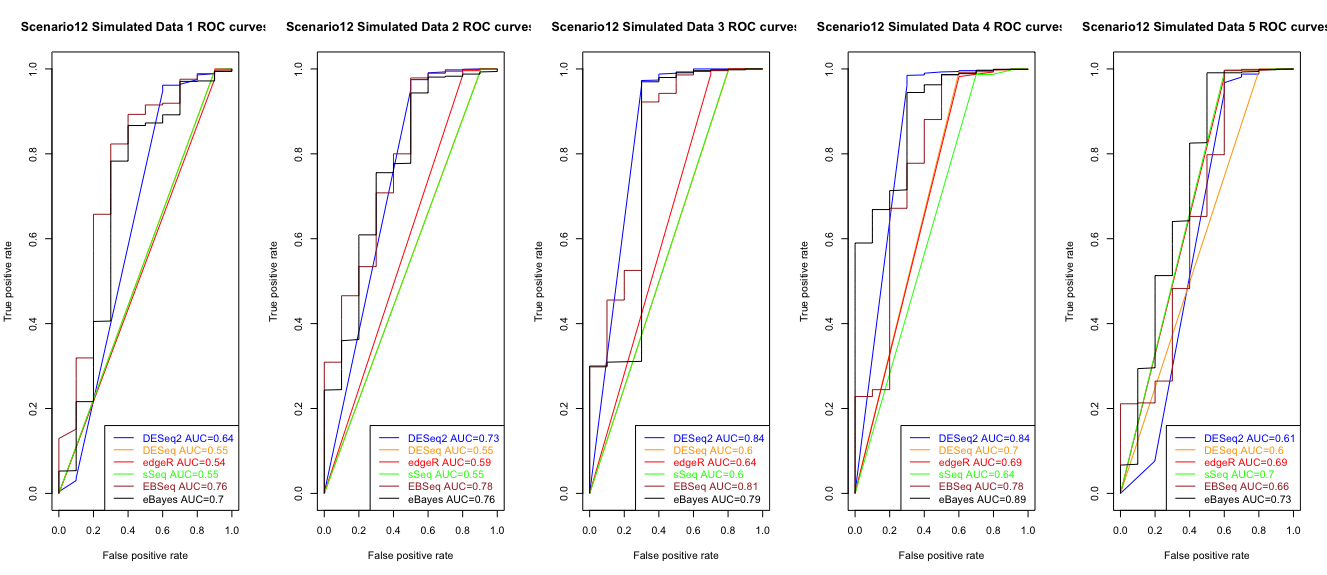
\includegraphics[height=6cm,width=15cm]{sc12_roc}
\caption{ROC curves of Simulated Datasets with $nGenes=1000, nSamples=8, pDiff=1\%$}
\label{sc12_roc}
\end{figure}


\begin{figure}[h!tb] 
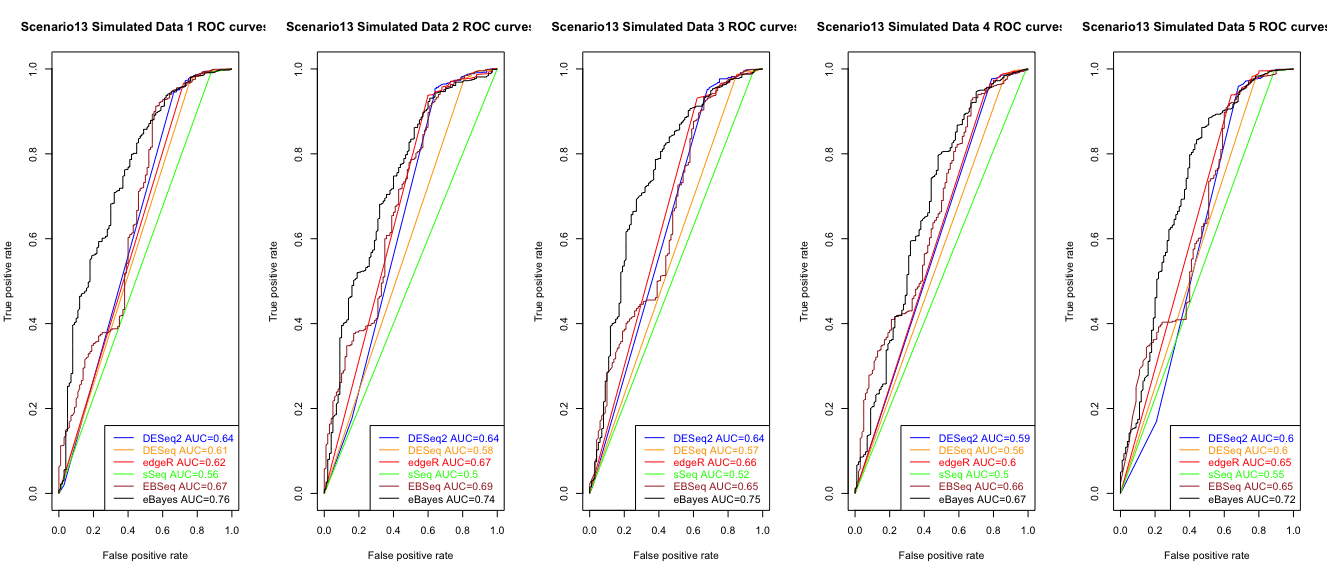
\includegraphics[height=6cm,width=15cm]{sc13_roc}
\caption{ROC curves of Simulated Datasets with $nGenes=1000, nSamples=4, pDiff=10\%$}
\label{sc13_roc}
\end{figure}


\begin{figure}[h!tb] 
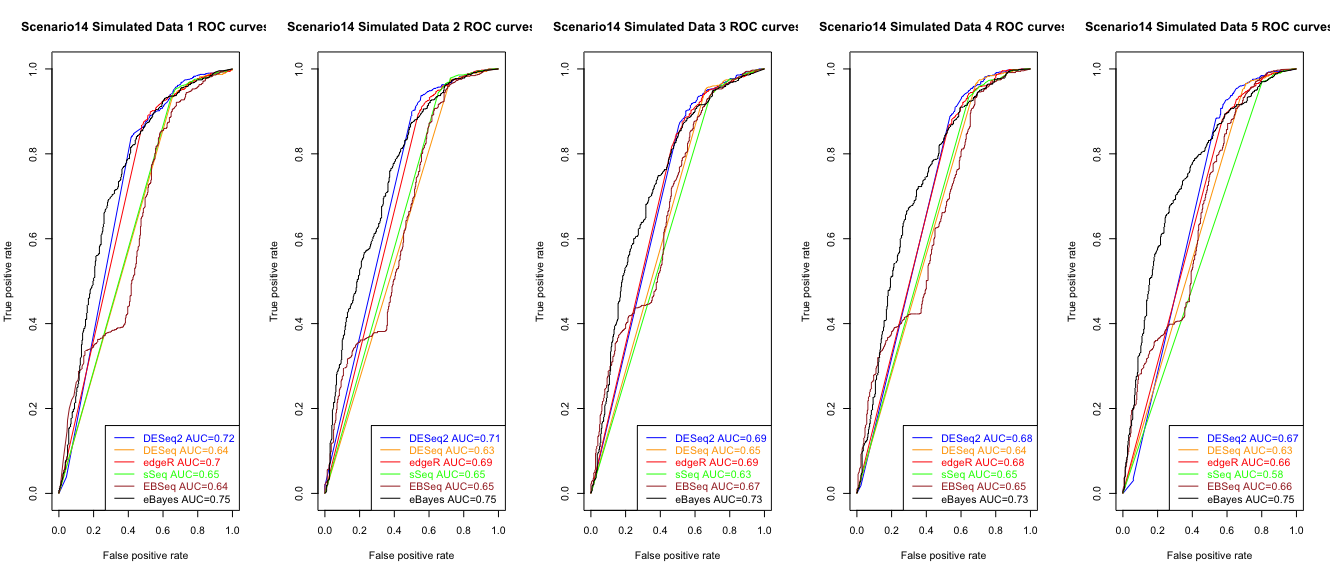
\includegraphics[height=6cm,width=15cm]{sc14_roc}
\caption{ROC curves of Simulated Datasets with $nGenes=1000, nSamples=4, pDiff=30\%$}
\label{sc14_roc}
\end{figure}


\begin{figure}[h!tb] 
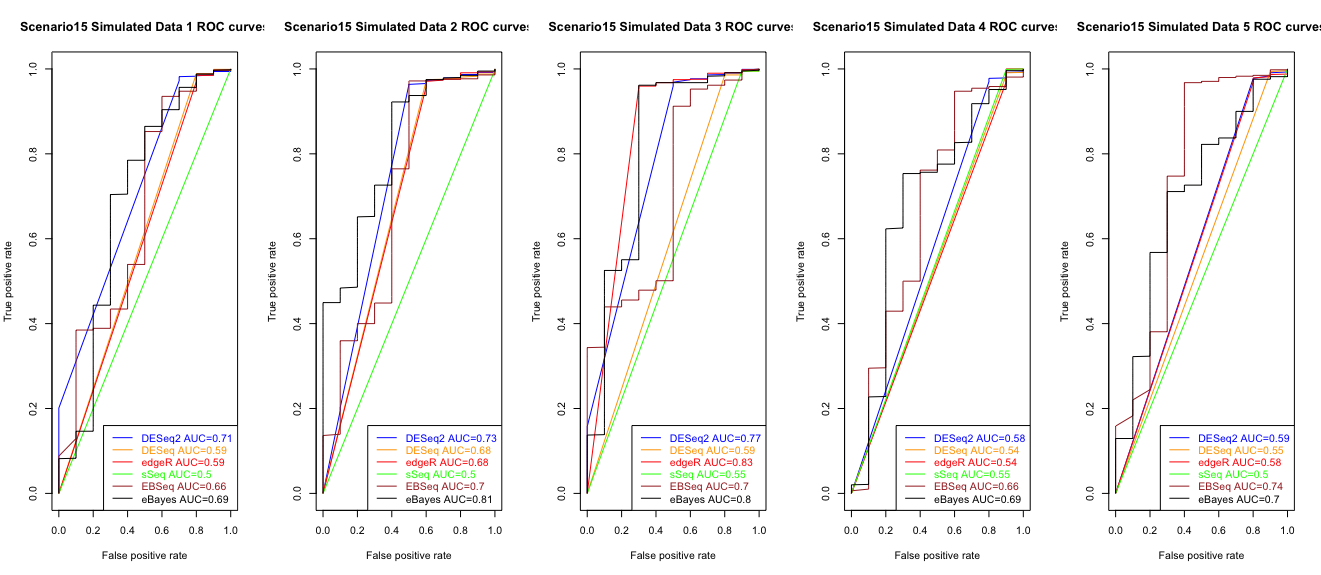
\includegraphics[height=6cm,width=15cm]{sc15_roc}
\caption{ROC curves of Simulated Datasets with $nGenes=1000, nSamples=4, pDiff=1\%$}
\label{sc15_roc}
\end{figure}

\begin{figure}[h!tb] 
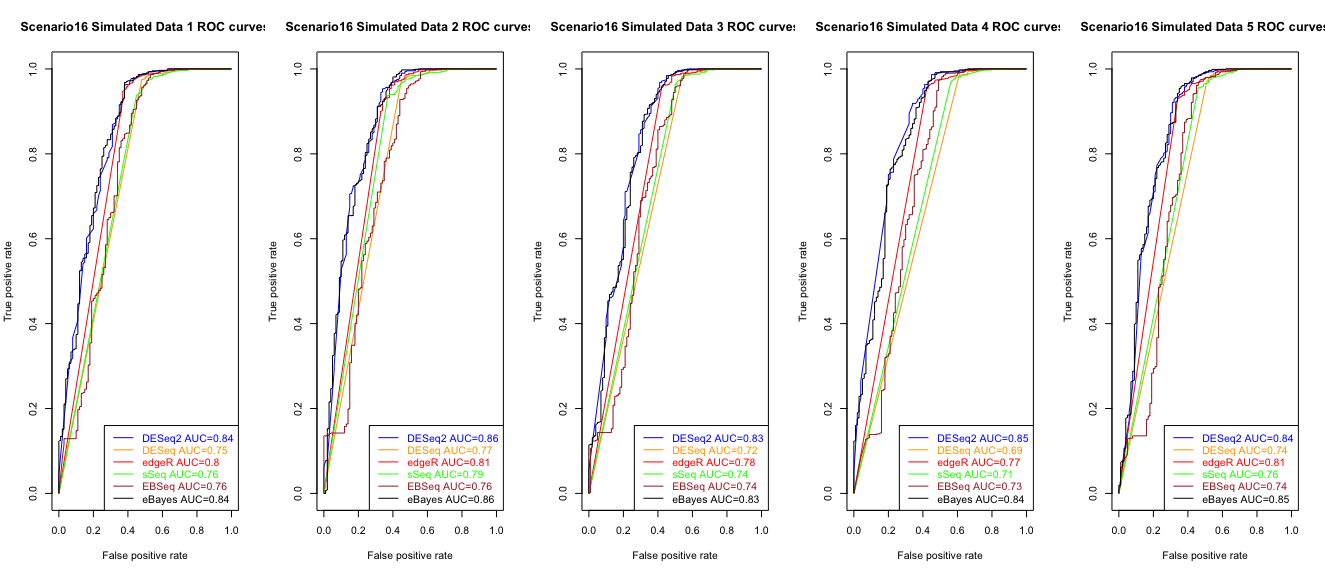
\includegraphics[height=6cm,width=15cm]{sc16_roc}
\caption{ROC curves of Simulated Datasets with $nGenes=1000, nSamples=16, pDiff=10\%$}
\label{sc16_roc}
\end{figure}

\begin{figure}[h!tb] 
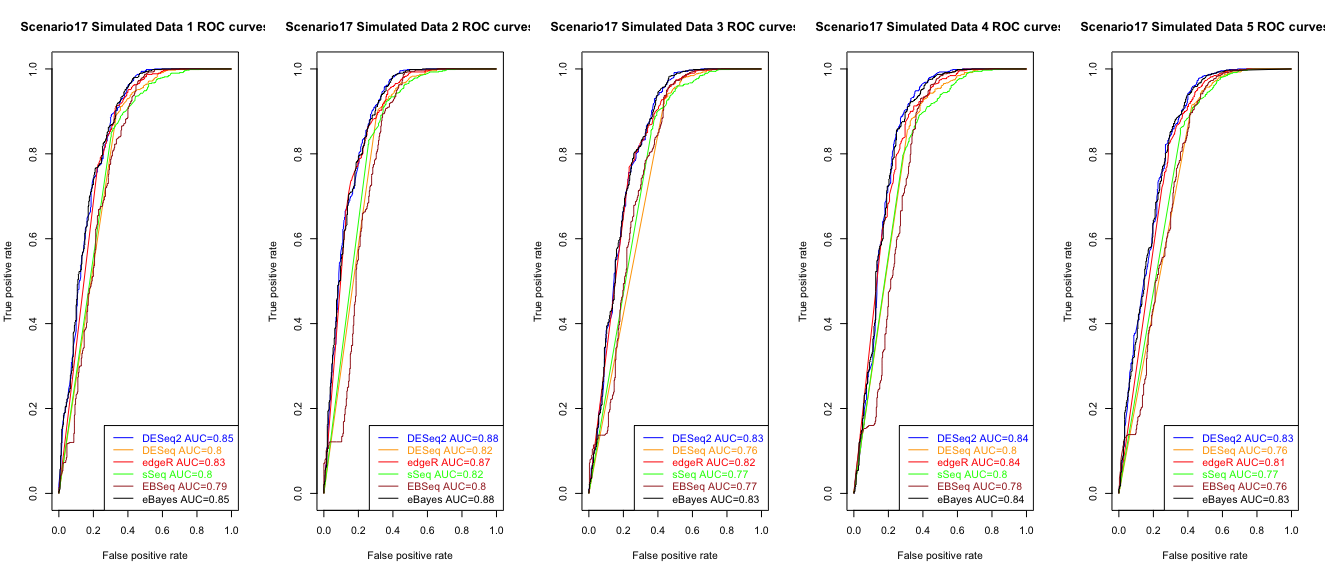
\includegraphics[height=6cm,width=15cm]{sc17_roc}
\caption{ROC curves of Simulated Datasets with $nGenes=1000, nSamples=16, pDiff=30\%$}
\label{sc17_roc}
\end{figure}

\begin{figure}[h!tb] 
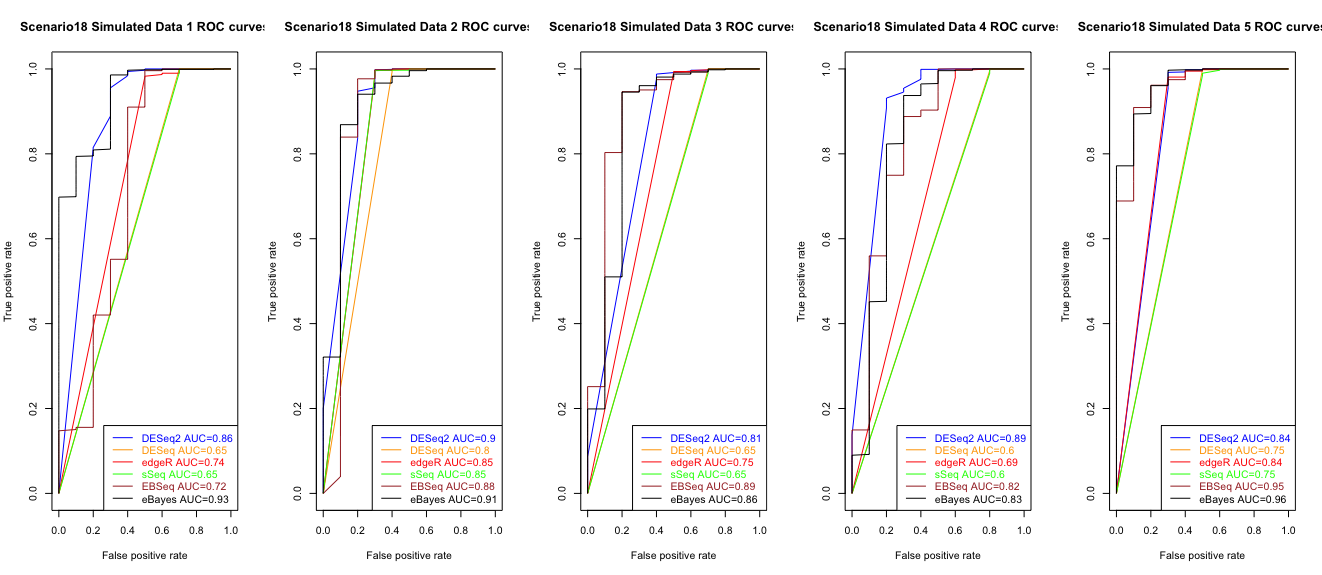
\includegraphics[height=6cm,width=15cm]{sc18_roc}
\caption{ROC curves of Simulated Datasets with $nGenes=1000, nSamples=16, pDiff=1\%$}
\label{sc18_roc}
\end{figure}